\chapter{Additional figures}
\label{sec:figures}

Here the plots and graphs not included on the main text are  included.

\begin{figure}
\begin{center}
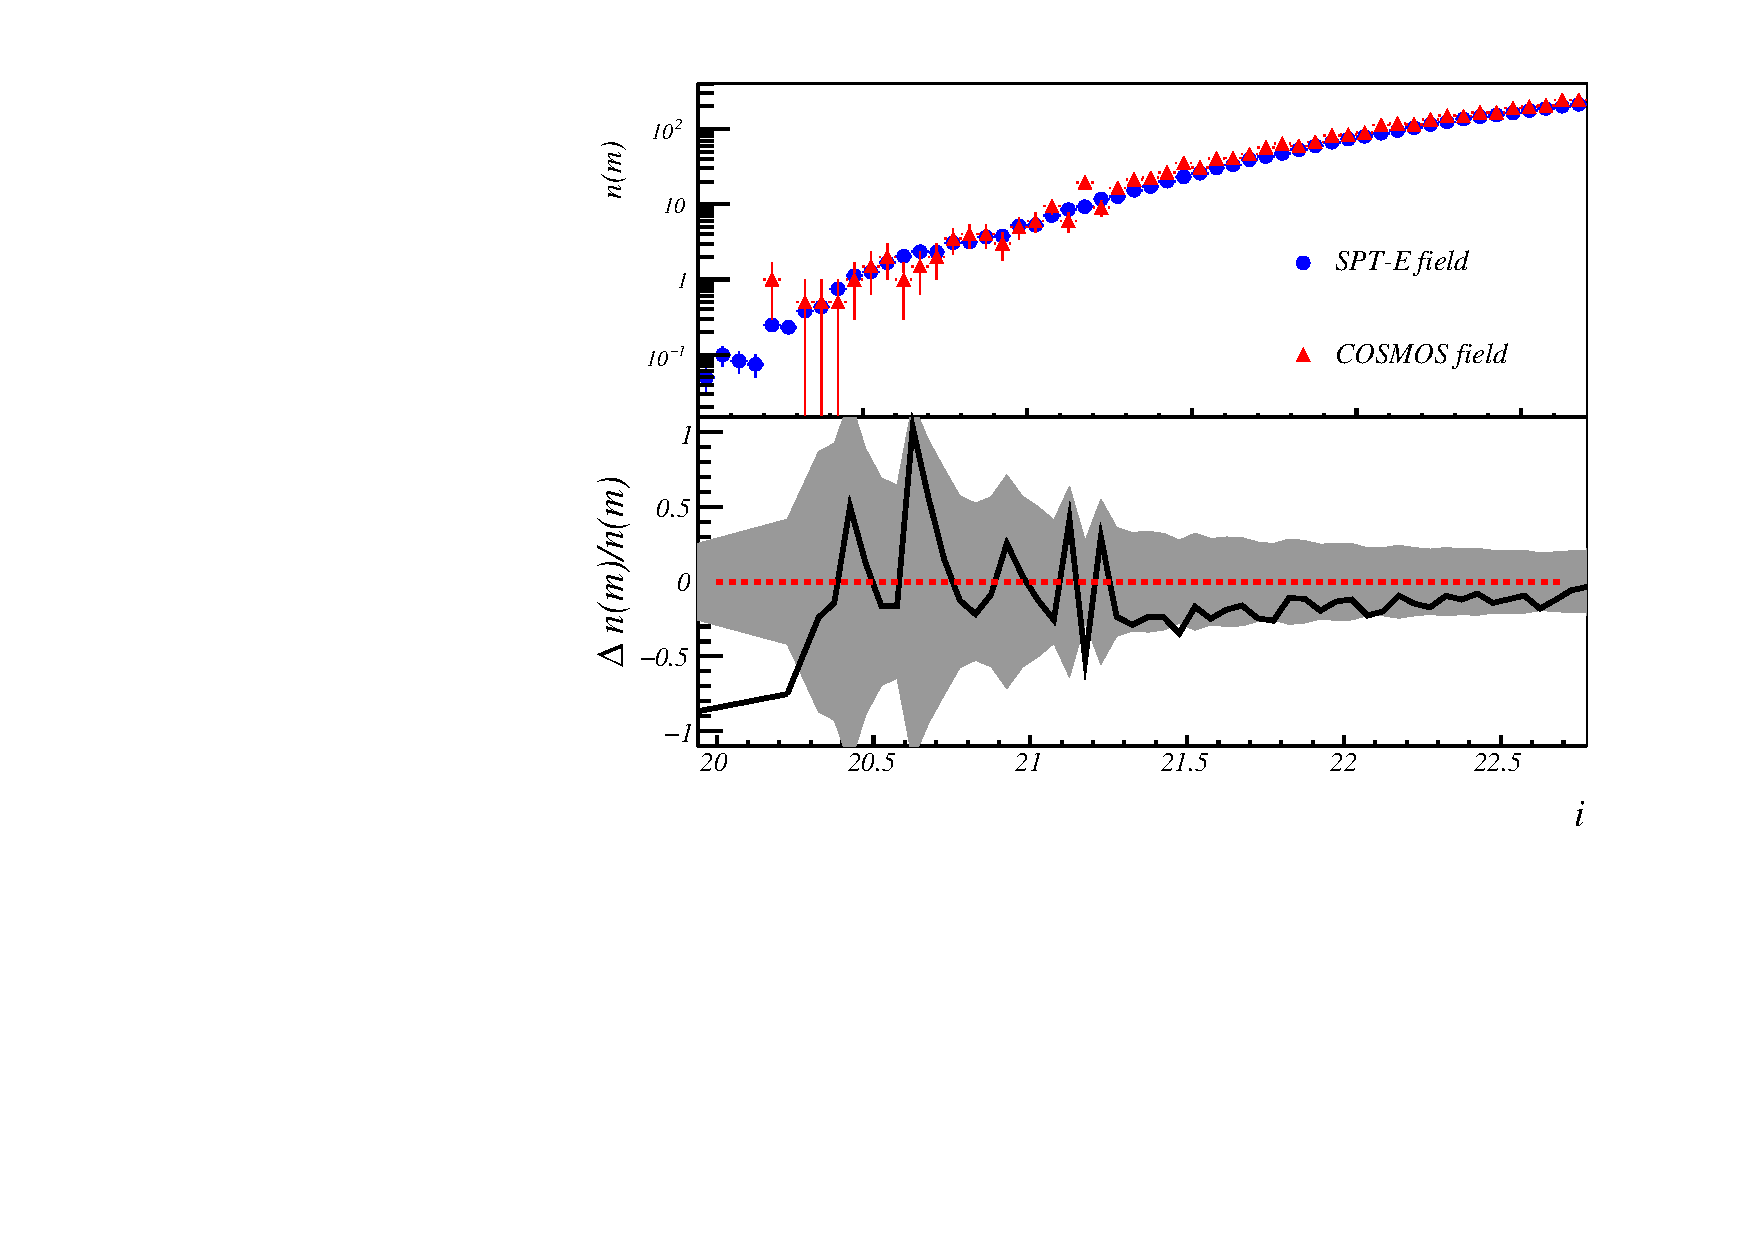
\includegraphics[width=0.85\textwidth]{./figures_appendix/SPTE_SNe_r.pdf}
\caption{Upper panel: Comparison of the magnitude distribution for the SPT-E and the COSMOS fields for the $r$ band.}
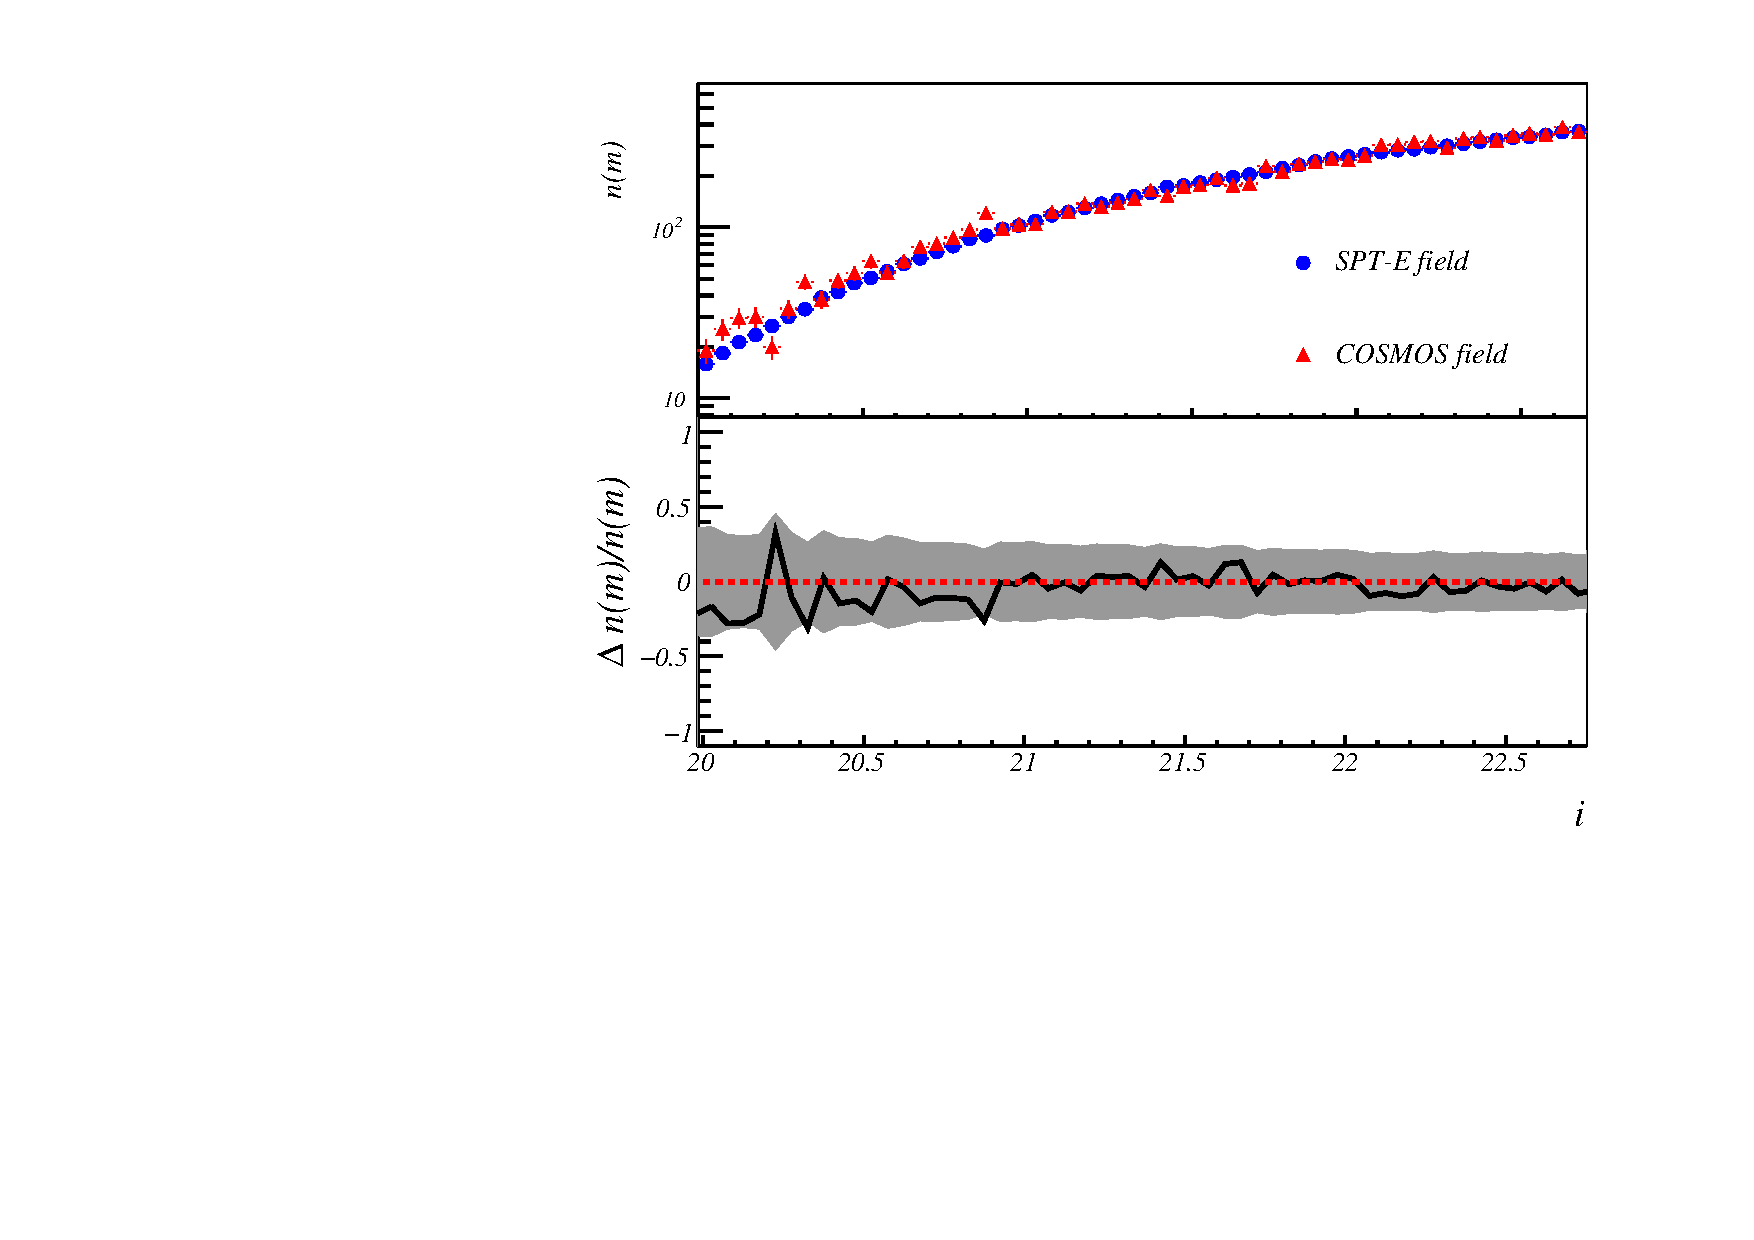
\includegraphics[width=0.85\textwidth]{./figures_appendix/SPTE_SNe_z.pdf}
\caption{Upper panel: Comparison of the magnitude distribution for the SPT-E and the COSMOS fields for the $z$ band.}
\end{center}
\end{figure}

\begin{sidewaysfigure}
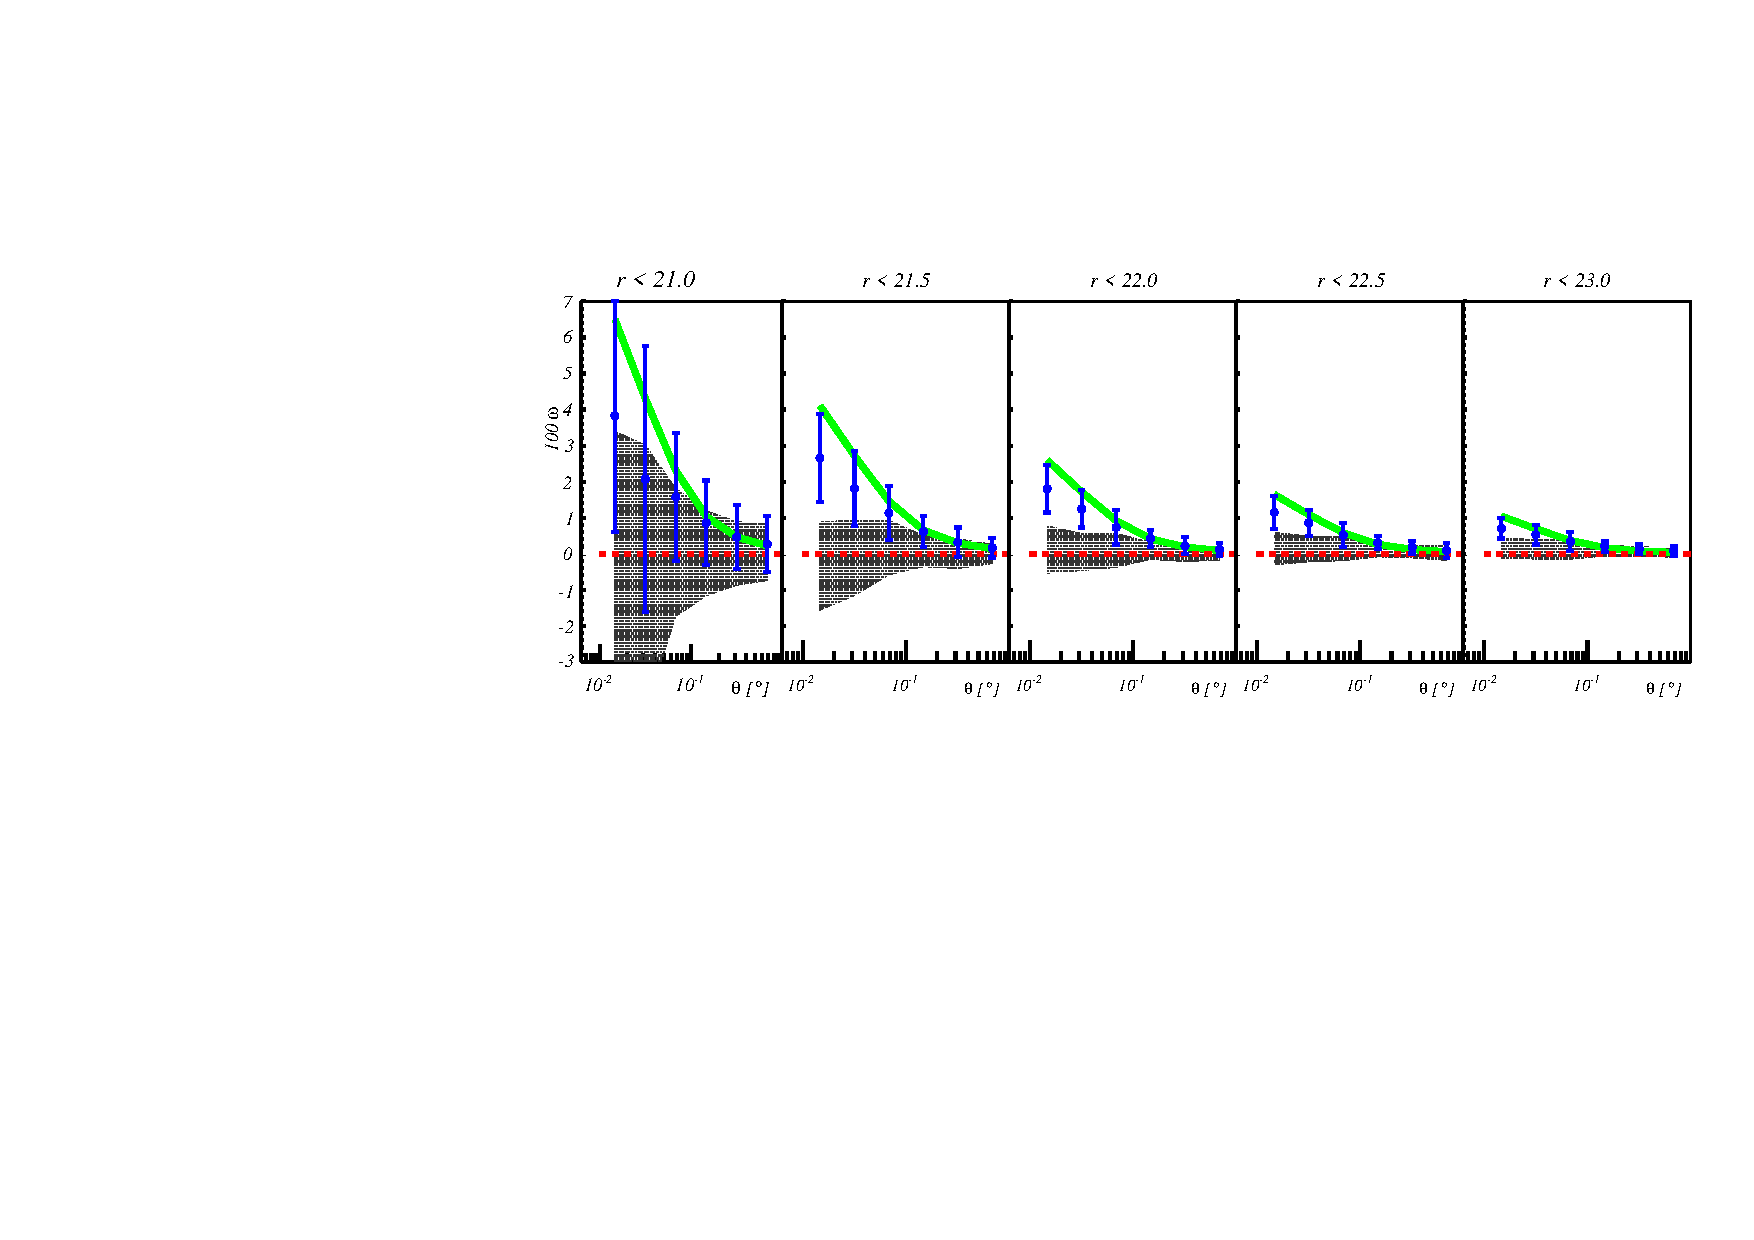
\includegraphics[width=\textwidth,trim={0 2.3cm 0 3.5cm},clip]{./figures_appendix/mag_r_MICE.pdf}
\caption{MICE $r$-band.}
\end{sidewaysfigure}

\begin{sidewaysfigure}
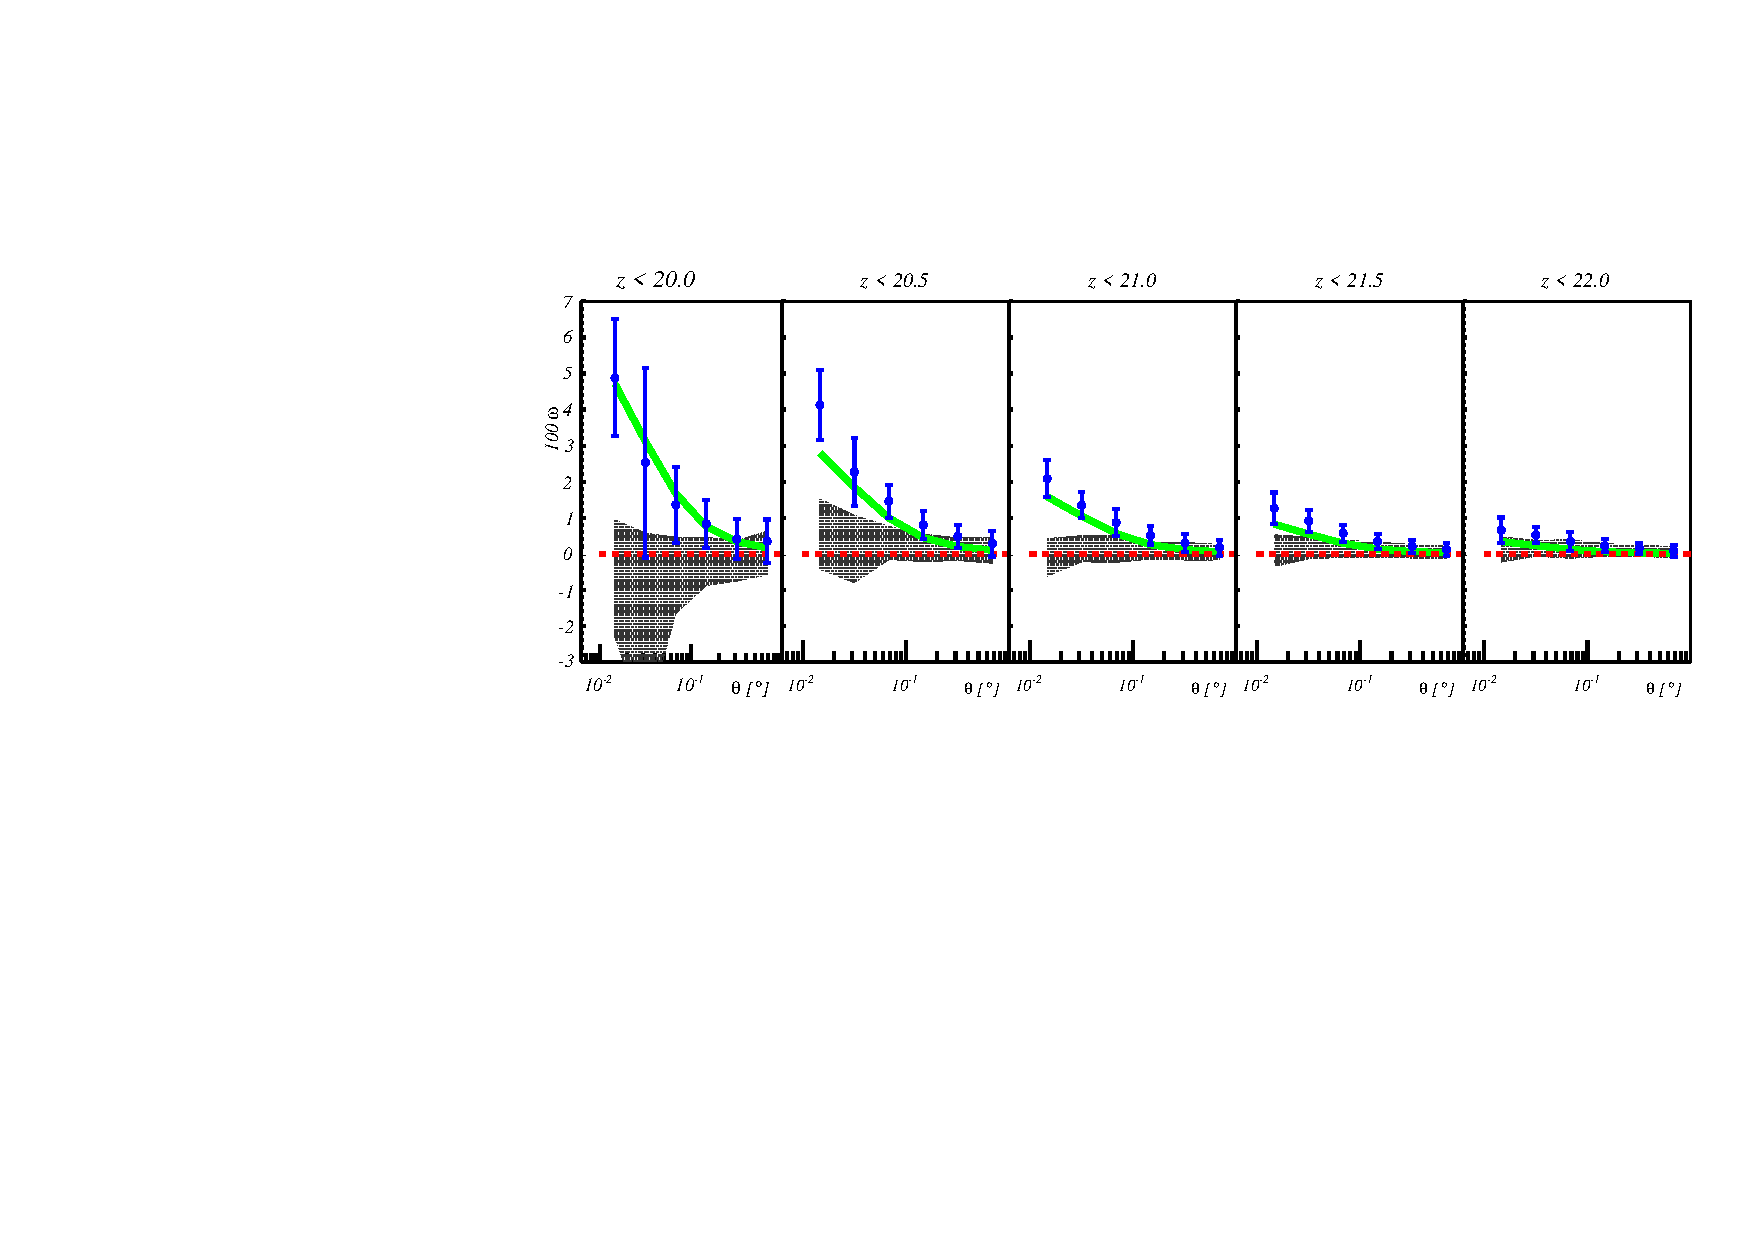
\includegraphics[width=\textwidth,trim={0 2.3cm 0 3.5cm},clip]{./figures_appendix/mag_z_MICE.pdf}
\caption{MICE $z$-band.}
\end{sidewaysfigure}

\begin{figure}
\begin{center}
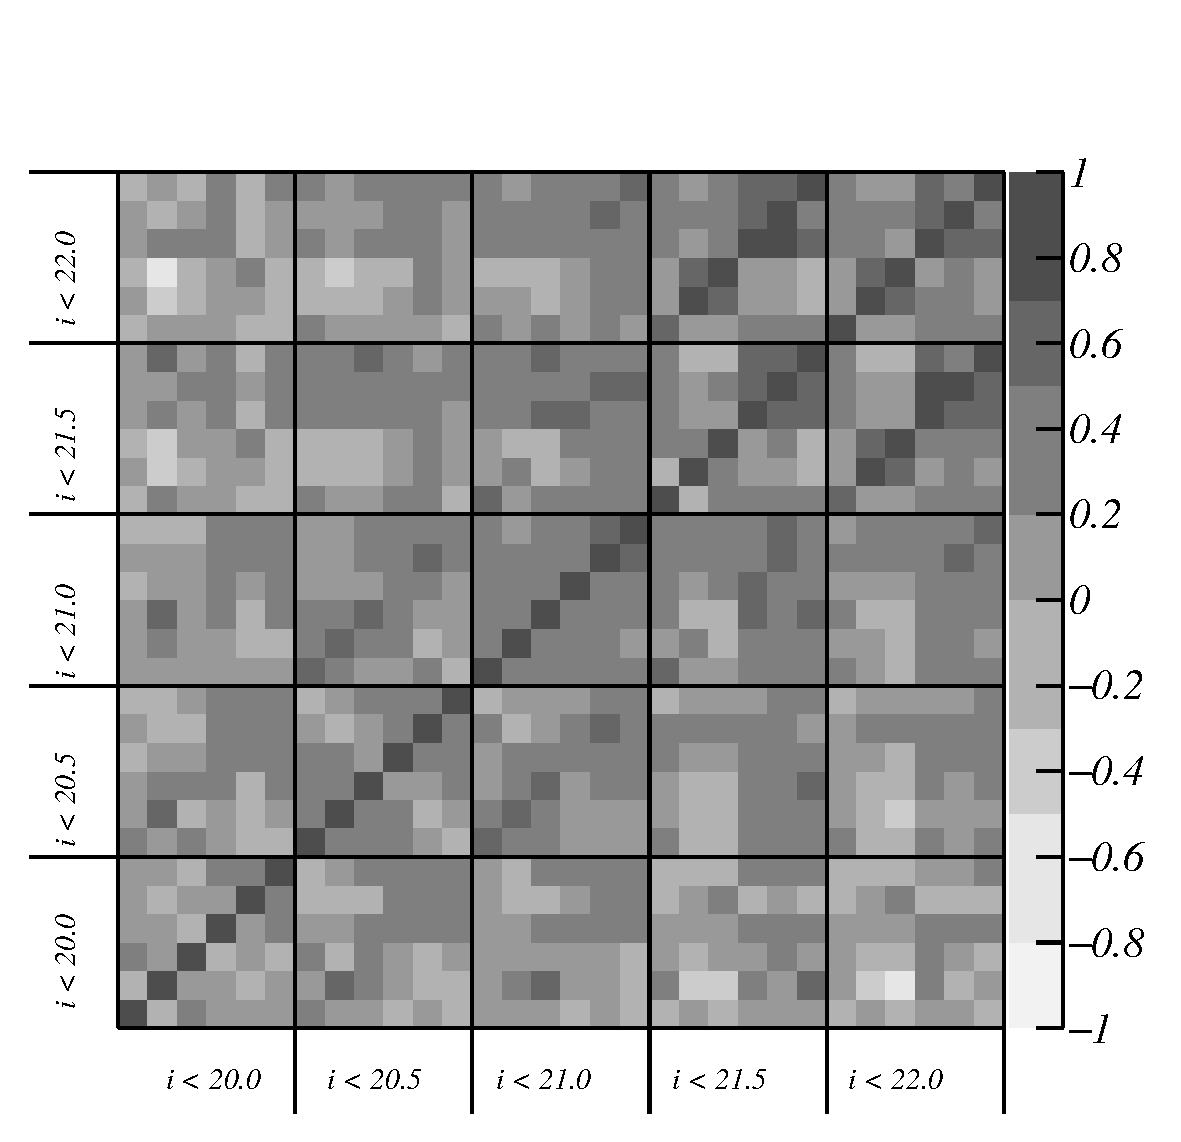
\includegraphics[width=0.8\textwidth,trim={0 0 0 2cm},clip]{./figures_appendix/cov_matrix_mag_auto_r.pdf}
\caption{Covariance matrix of the {\it r}-band rescaled by the value of the diagonal.}
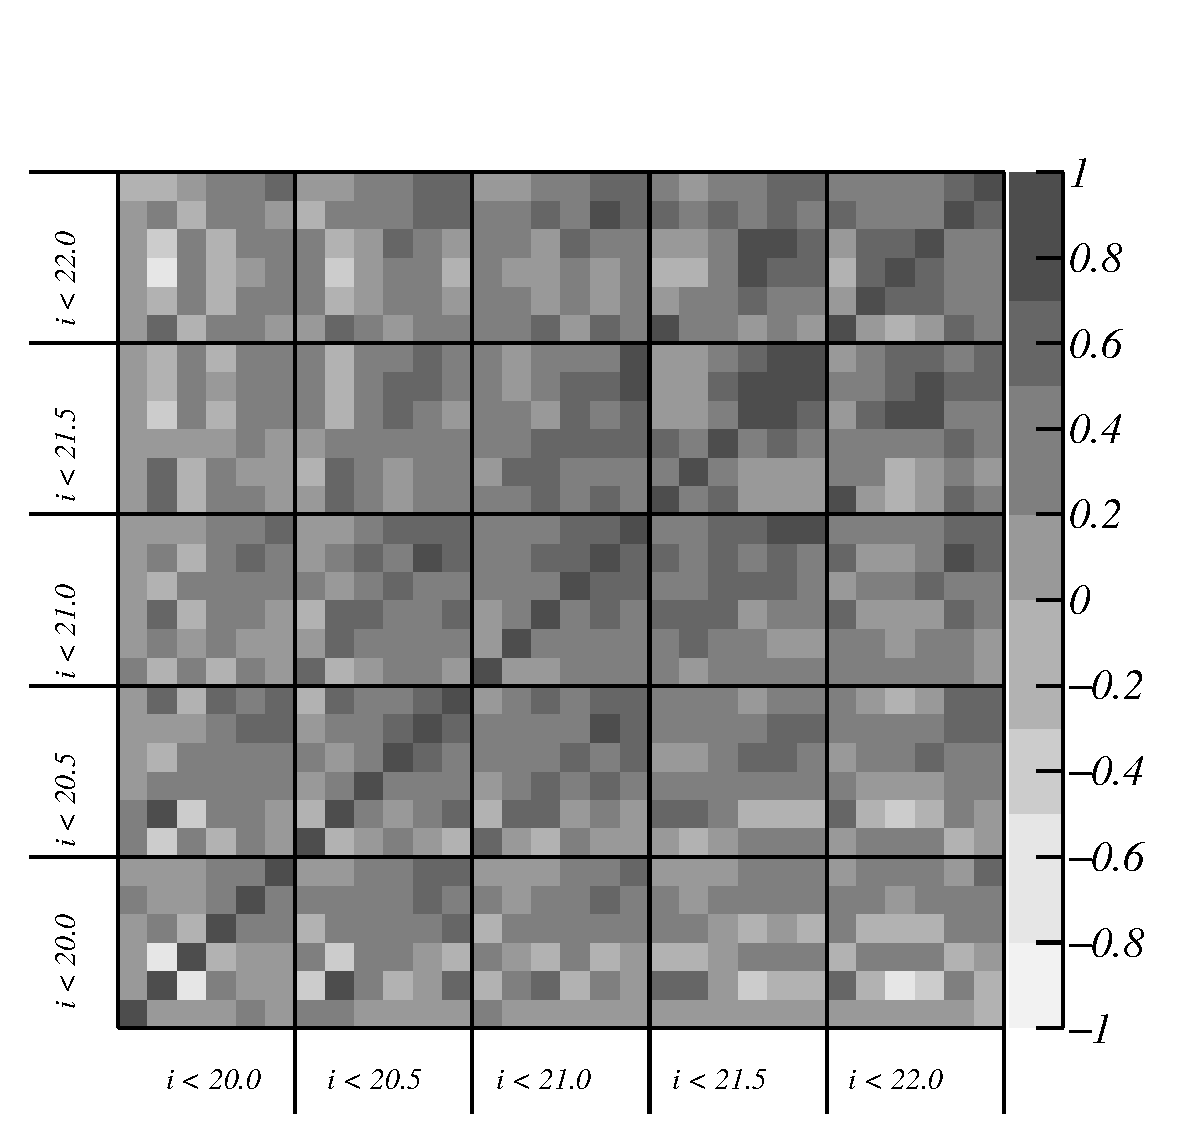
\includegraphics[width=0.8\textwidth,trim={0 0 0 2cm},clip]{./figures_appendix/cov_matrix_mag_auto_z.pdf}
\caption{Covariance matrix of the {\it z}-band rescaled by the value of the diagonal.}
\end{center}
\end{figure}

\begin{sidewaysfigure}
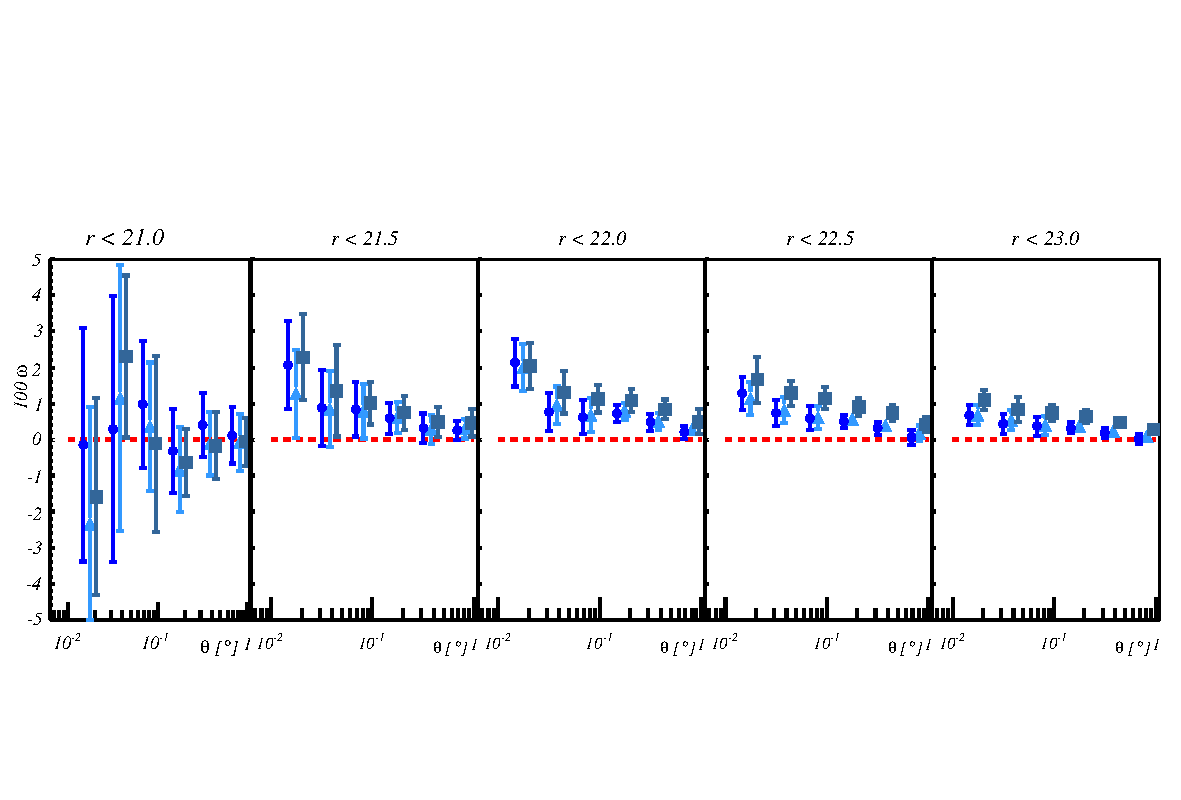
\includegraphics[width=\textwidth,trim={0 2.3cm 0 3.5cm},clip]{./figures_appendix/mag_r_photoz_comparison.pdf}
\caption{DES-SV $r$-band photo-z comparison.}
\end{sidewaysfigure}

\begin{sidewaysfigure}
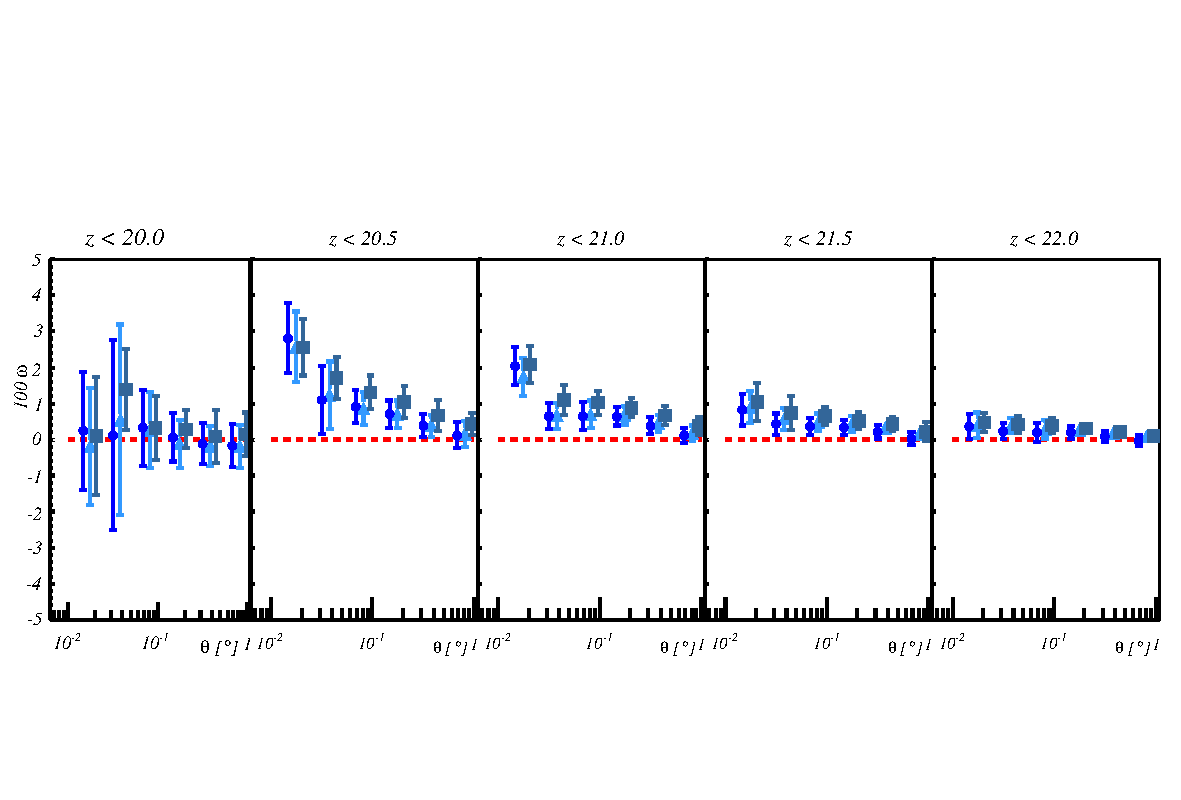
\includegraphics[width=\textwidth,trim={0 2.3cm 0 3.5cm},clip]{./figures_appendix/mag_z_photoz_comparison.pdf}
\caption{DES-SV $z$-band photo-z comparison.}
\end{sidewaysfigure}

\begin{sidewaysfigure}
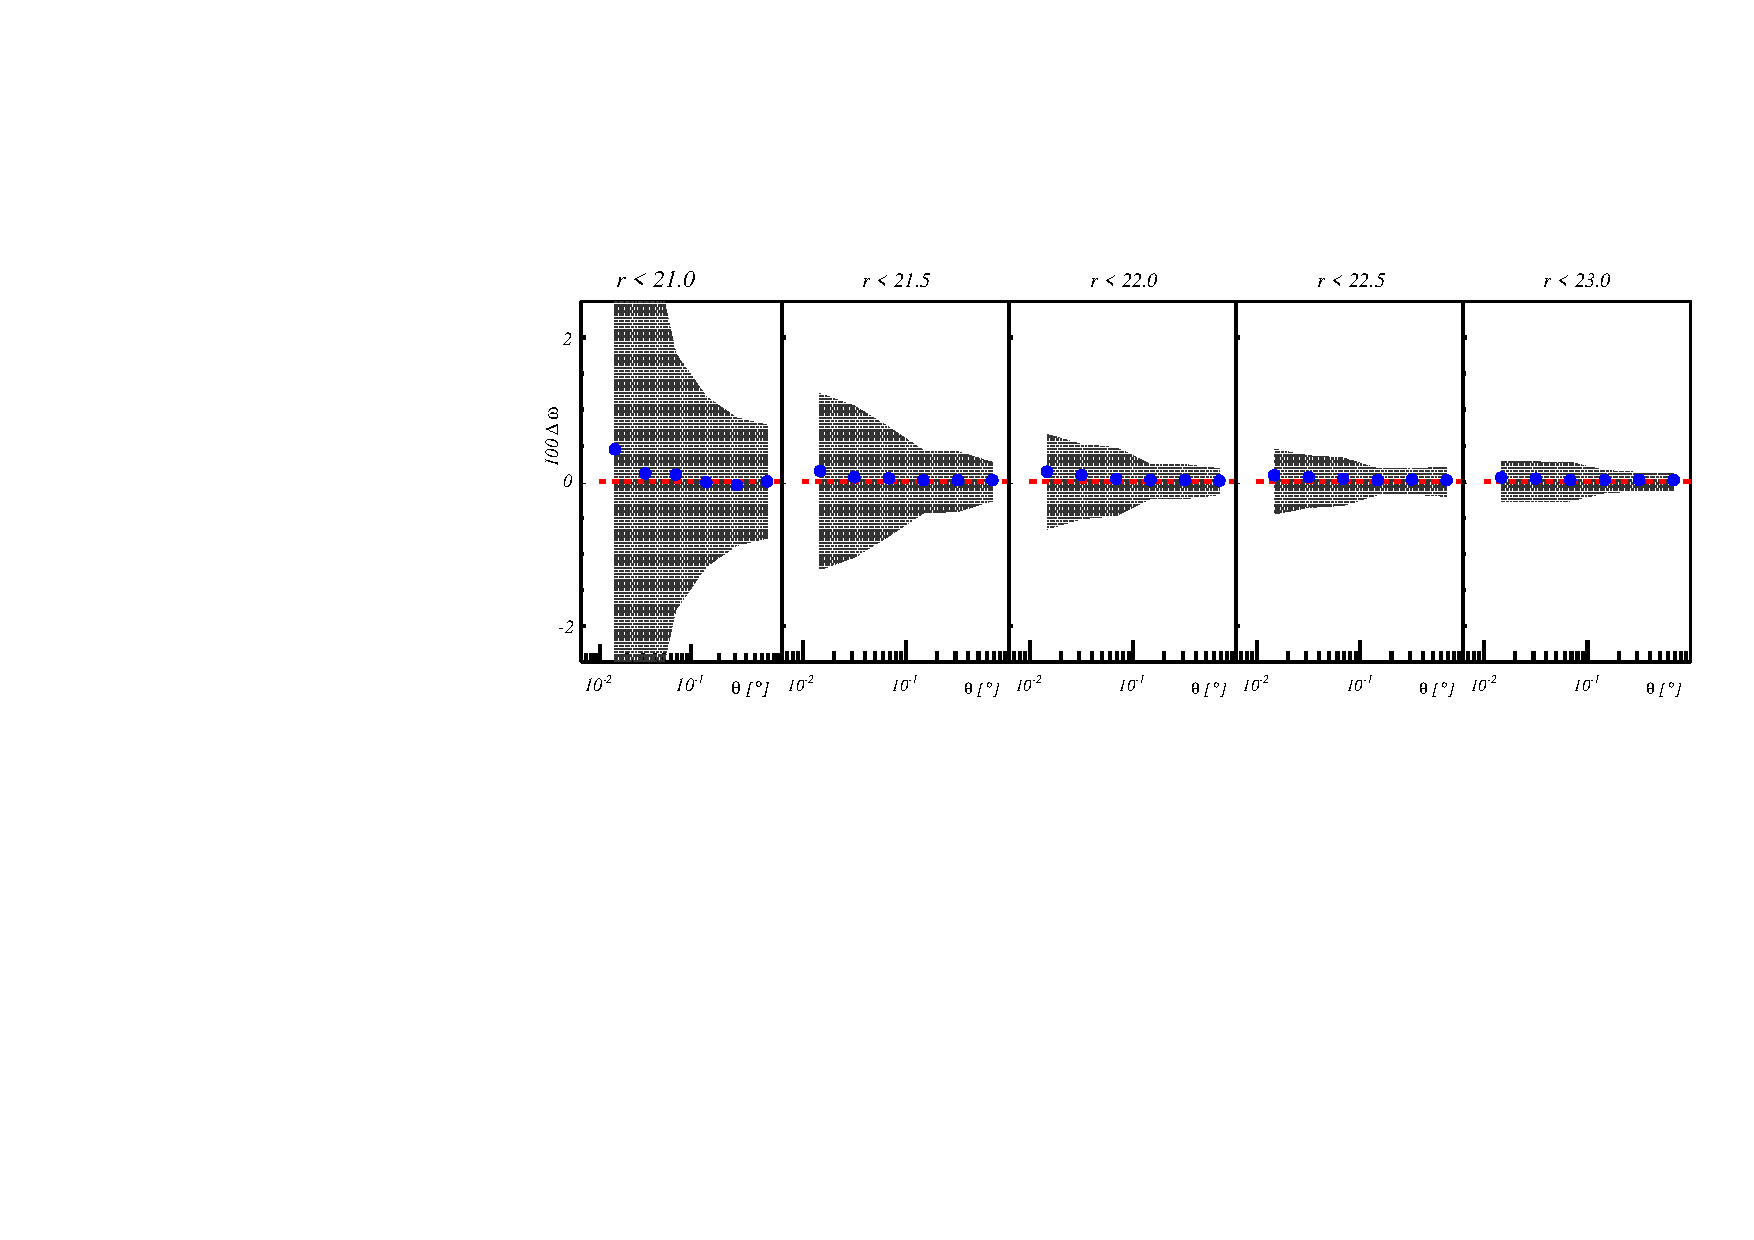
\includegraphics[width=\textwidth,trim={0 2.3cm 0 3.5cm},clip]{./figures_appendix/mag_rdust.pdf}
\caption{DES-SV $r$-band estimation of dust extinction with MICE.}
\end{sidewaysfigure}

\begin{sidewaysfigure}
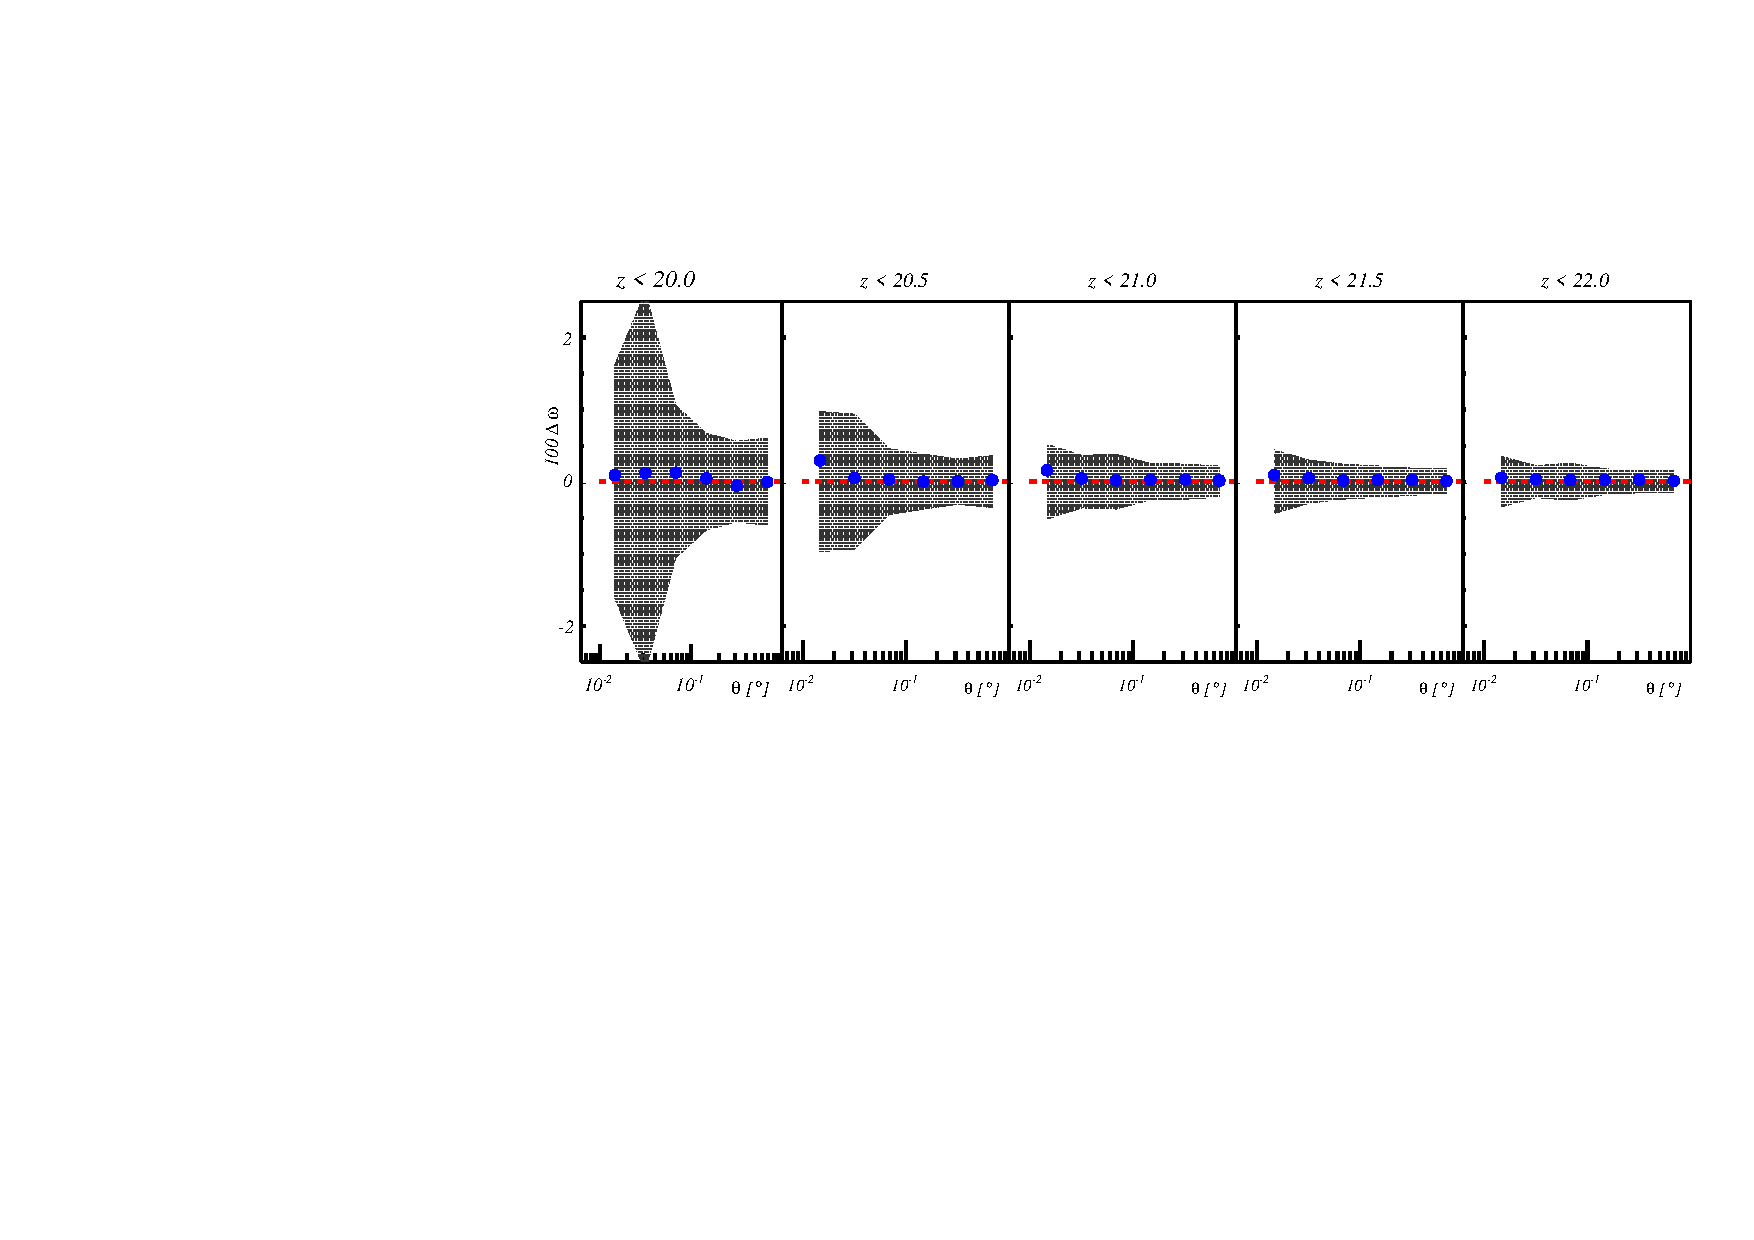
\includegraphics[width=\textwidth,trim={0 2.3cm 0 3.5cm},clip]{./figures_appendix/mag_zdust.pdf}
\caption{DES-SV $z$-band estimation of dust extinction with MICE.}
\end{sidewaysfigure}

\begin{sidewaysfigure}
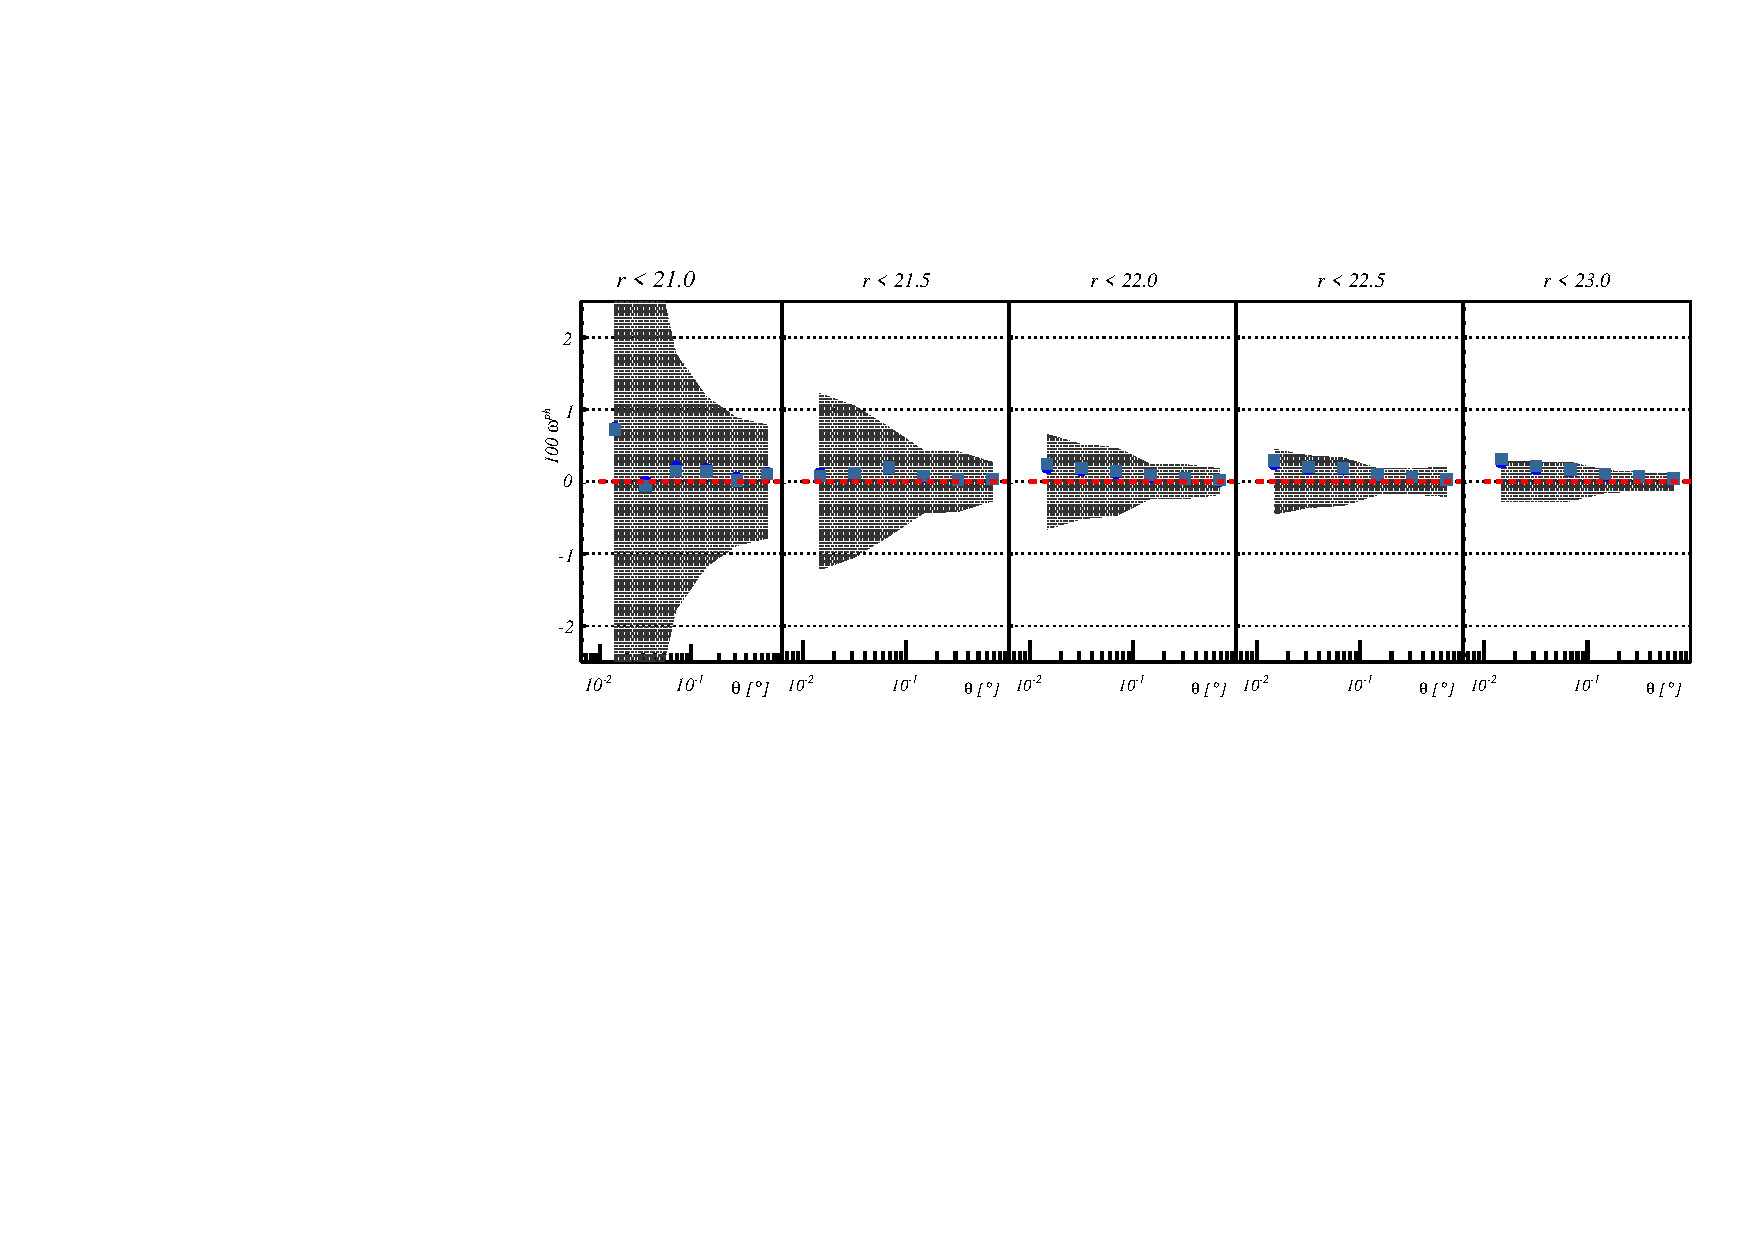
\includegraphics[width=\textwidth,trim={0 2.3cm 0 3.5cm},clip]{./figures_appendix/mag_r_mix.pdf}
\caption{DES-SV $z$-band estimation of photo-z induced signal with MICE.}
\end{sidewaysfigure}

\begin{sidewaysfigure}
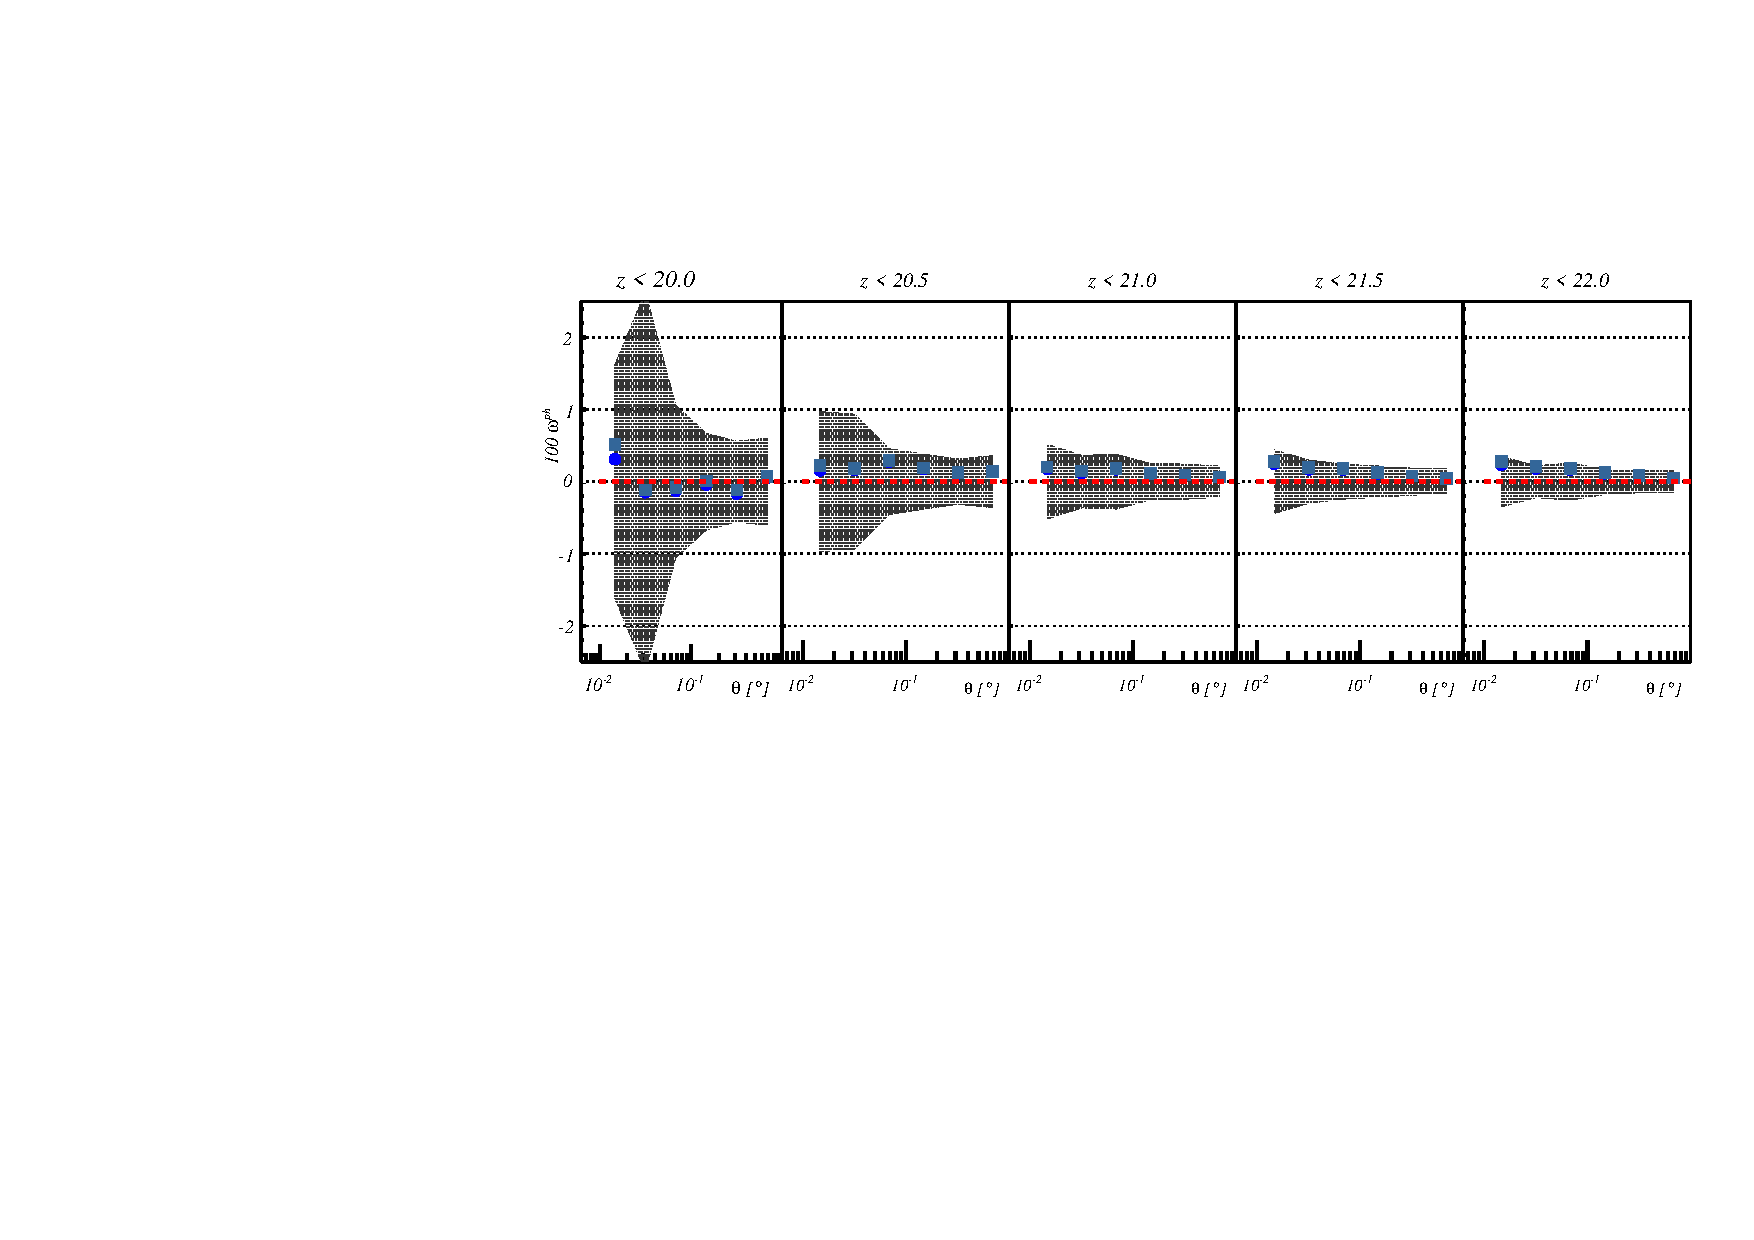
\includegraphics[width=\textwidth,trim={0 2.3cm 0 3.5cm},clip]{./figures_appendix/mag_z_mix.pdf}
\caption{DES-SV $z$-band estimation of photo-z induced signal with MICE.}
\end{sidewaysfigure}

\begin{sidewaysfigure}
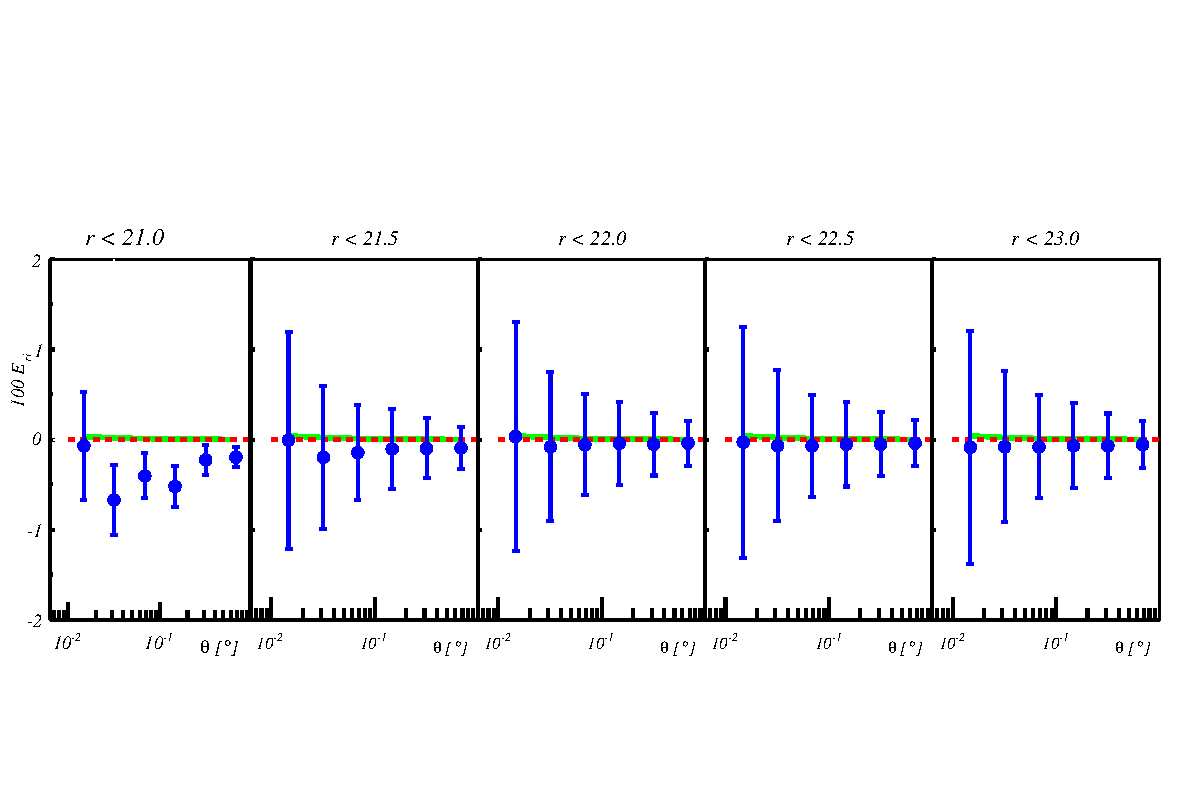
\includegraphics[width=\textwidth,trim={0 2.3cm 0 3.5cm},clip]{./figures_appendix/mag_r_ri.pdf}
\caption{DES-SV $r$-band estimation of the $r-i$ color excess.}
\end{sidewaysfigure}

\begin{sidewaysfigure}
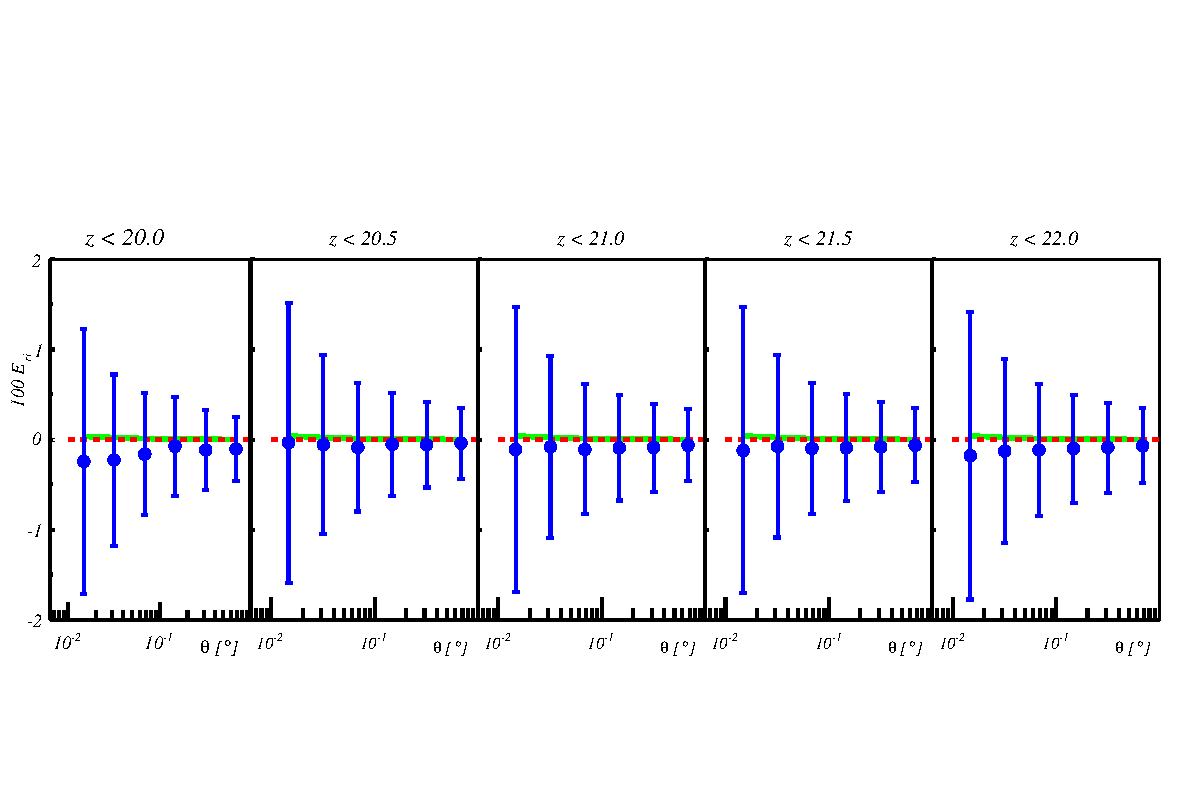
\includegraphics[width=\textwidth,trim={0 2.3cm 0 3.5cm},clip]{./figures_appendix/mag_z_ri.pdf}
\caption{DES-SV $z$-band estimation of the $r-i$ color excess.}
\end{sidewaysfigure}

\begin{sidewaysfigure}
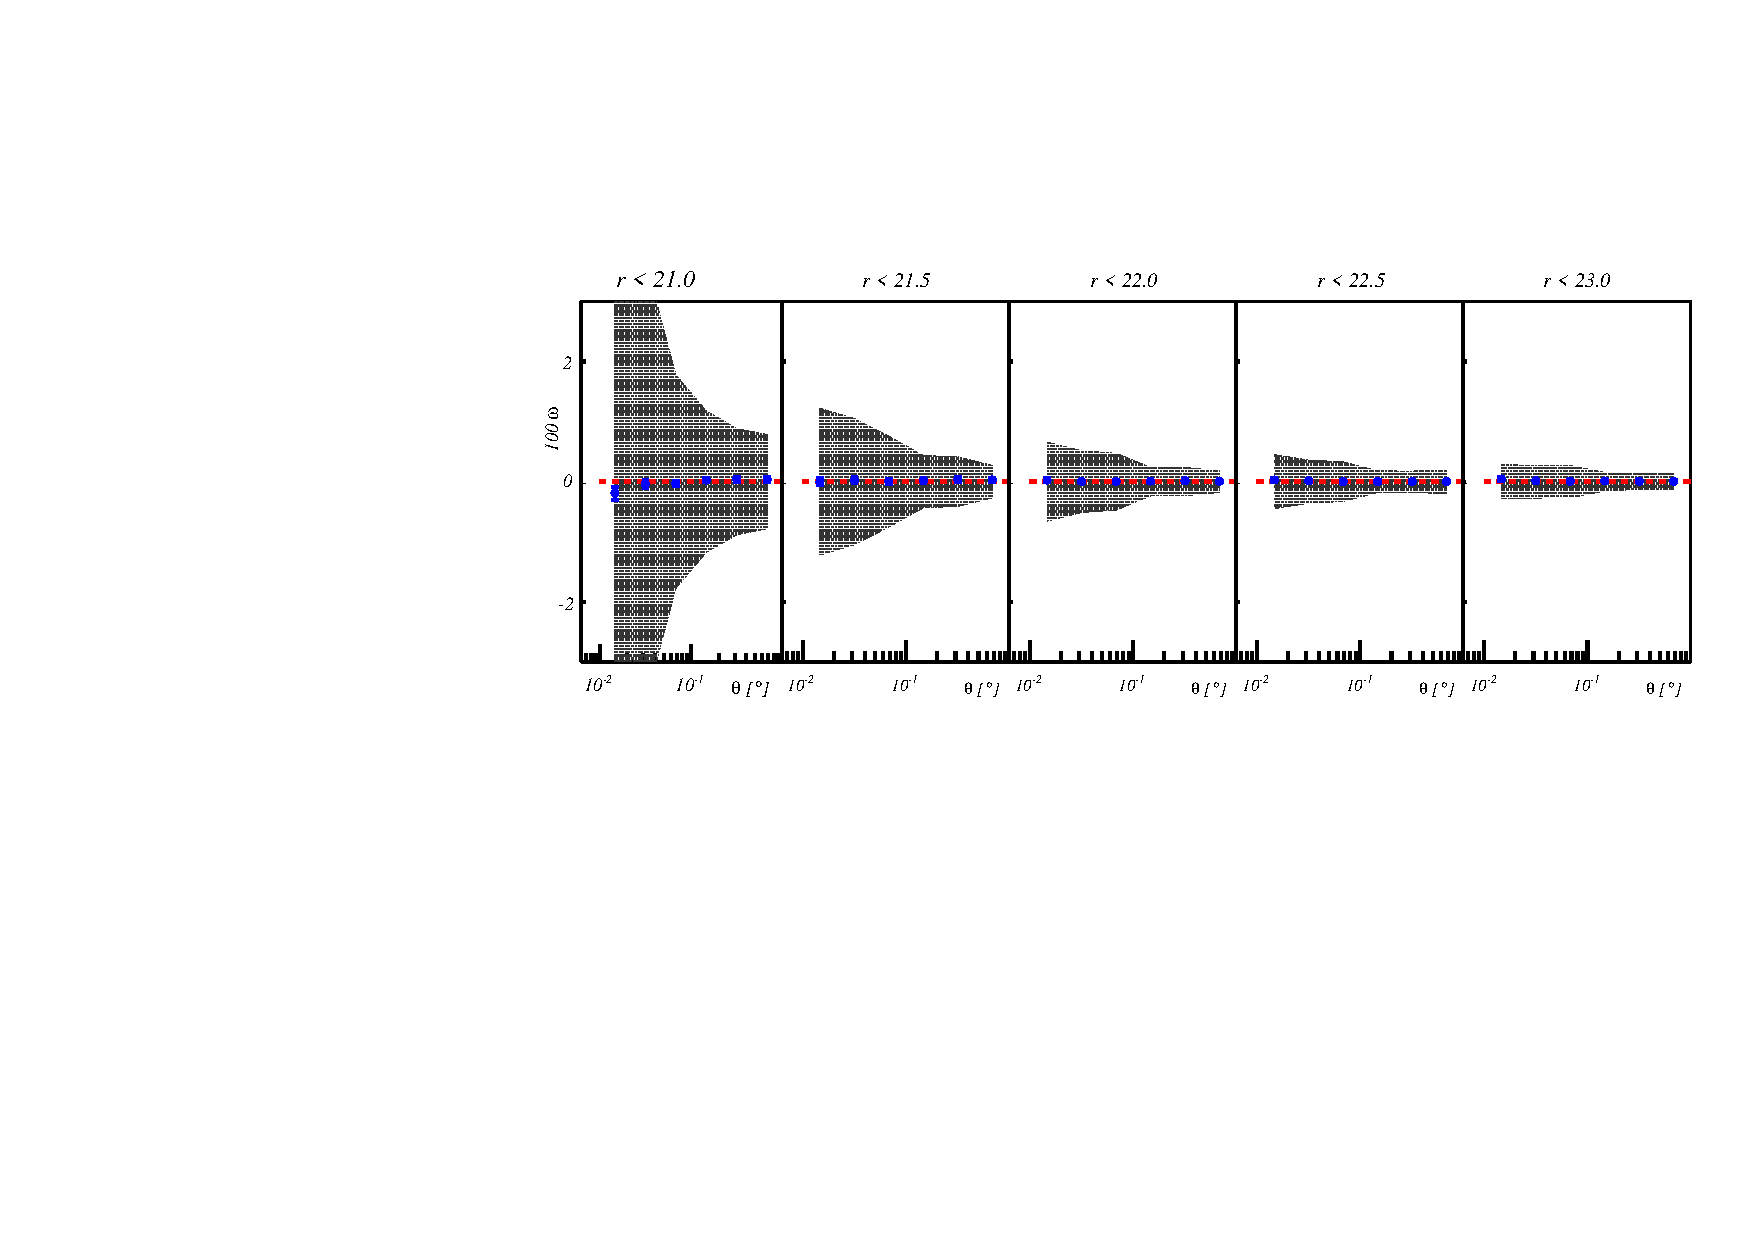
\includegraphics[width=\textwidth,trim={0 2.3cm 0 3.5cm},clip]{./figures_appendix/mag_rstars.pdf}
\caption{DES-SV $r$-band estimation of the signal induced by stellar contamination.}
\end{sidewaysfigure}

\begin{sidewaysfigure}
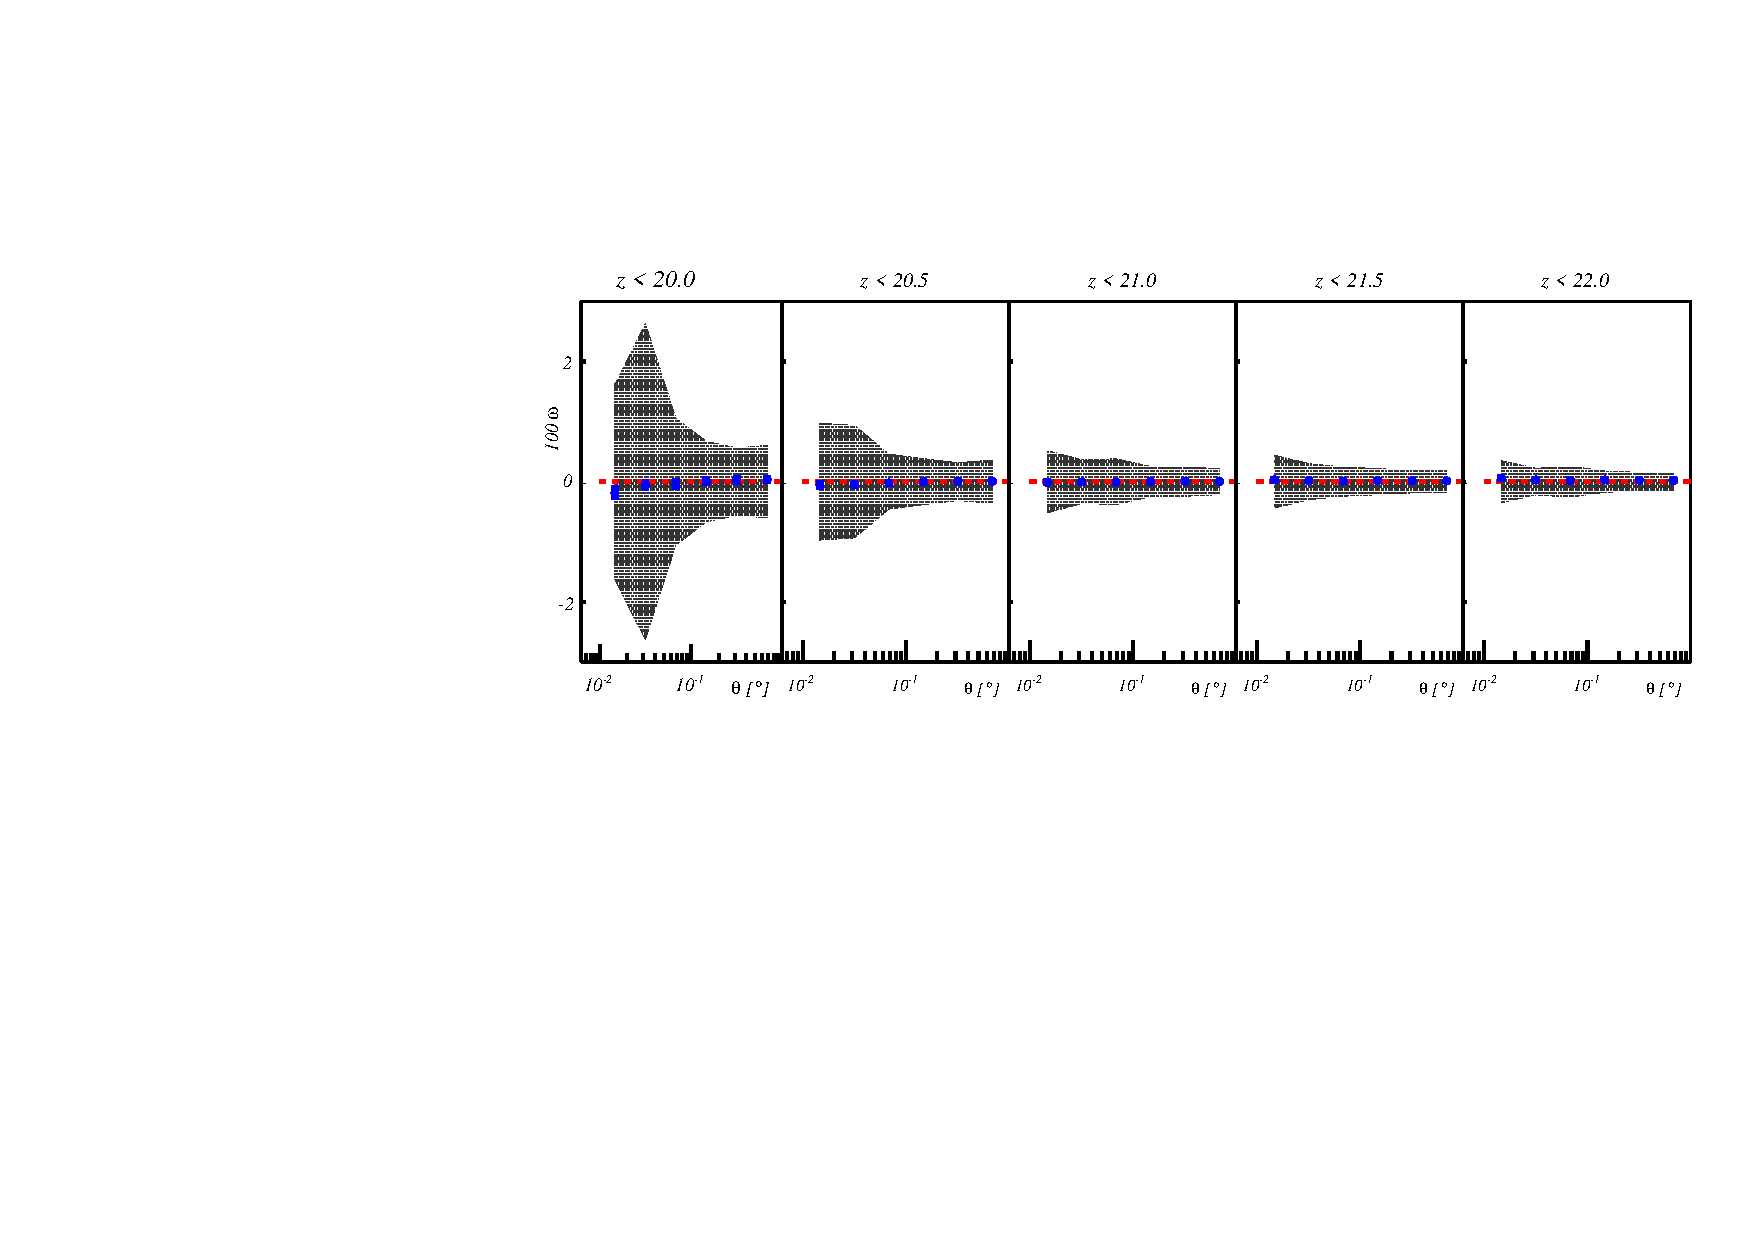
\includegraphics[width=\textwidth,trim={0 2.3cm 0 3.5cm},clip]{./figures_appendix/mag_zstars.pdf}
\caption{DES-SV $z$-band estimation of the signal induced by the stellar contamination.}
\end{sidewaysfigure}